\chapter{Aplikacja internetowa}
\section{Architektura aplikacji} % (fold)
\label{sec:architektura_aplikacji}

\subsection{Wzorzec Model-Widok-Kontroler} % (fold)
\label{sub:wzorzec_model_widok_kontroler}
\paragraph{} % (fold)
\label{par:paragraph_name}
Model-Widok-Kontroler (\textit{ang. Model-View-Controller}) w skrócie MVC, jest wzorcem projektowym rozdzielający aplikację internetową na 3 warstwy : model, widok i kontroler. 

\subsubsection{Model}
\paragraph{}
Warstwa modelu odpowiada za reprezentację logiki systemu oraz dostęp do bazy danych. W projekcie za tę część aplikacji odpowiadają dwie biblioteki DLL : PI.Service oraz PI.Data.

\subsubsection{Widok}
\paragraph{}
Widok jest warstwą odpowiedzialną za wyświetlanie interfejsu użytkownika. Najczęściej widoki generowane są na podstawie modelu. W apliakcjach MVC widoki tylko wyświetlają informacje. Ta warstwa znajduje się w bibliotece PI.Web.

\subsubsection{Kontroler}
\paragraph{} 
Kontrolery to komponenty odpowiedzialne za utrzymanie interakcji z użytkownikiem, pracę z modelem i renderowaniem odpowiednich widoków. Kontrolery obsługują rządania użytkowników, konwertują parametry zapytań na modele i przekazują je do kolejnej warstwy. KOntrolery, podobnie jka widoki znajdują się w bibliotece PI.Web.  

\newpage
\begin{figure}[ht]
	\centering
		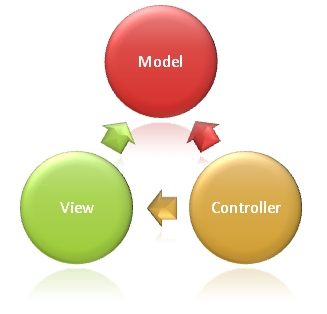
\includegraphics[width=0.5\linewidth]{assets/03_1.jpg}
	\caption{Schemat graficzny wzorca Model-Widok-Kontroler}
	\label{fig:kanji-giri}
\end{figure}

\subsection{Wzorzec Repozytorium} % (fold)
\label{sub:wzorzec_repozytorium}

% subsection wzorzec_repozytorium (end)

\subsection{Odwrócenie sterowania} % (fold)
\label{sub:odwr_cenie_sterowania}

% subsection odwr_cenie_sterowania (end)
% section architektura_aplikacji (end)